% !TEX program = pdflatex
\documentclass[10pt,aspectratio=169]{beamer}

\usepackage[utf8]{inputenc}
\usepackage[T1]{fontenc}
\usepackage[english]{babel}
\usepackage{lmodern}
\usepackage{microtype}
\usepackage{amsmath,amssymb,bm,mathtools}
\usepackage{booktabs,array}
\usepackage{tikz}

\usetheme[numbering=fraction,progressbar=frametitle]{metropolis}
\setbeamertemplate{frame numbering}[fraction]
\setbeamertemplate{navigation symbols}{}

\definecolor{CourseBlue}{HTML}{1A3C68}
\definecolor{CourseGreen}{HTML}{216E39}
\definecolor{CourseGold}{HTML}{B8860B}
\definecolor{CourseRed}{HTML}{9A2C2C}
\definecolor{SoftBlue}{HTML}{F2F6FA}
\definecolor{SoftGreen}{HTML}{F1F8F3}
\definecolor{SoftRed}{HTML}{FFF3F3}

\setbeamercolor{normal text}{fg=black,bg=white}
\setbeamercolor{structure}{fg=CourseBlue}
\setbeamercolor{title}{fg=CourseBlue}
\setbeamerfont{title}{size=\Large,series=\bfseries}
\setbeamercolor{frametitle}{bg=CourseBlue,fg=white}
\setbeamerfont{frametitle}{series=\bfseries,size=\large}
\setbeamertemplate{frametitle}{
  \nointerlineskip
  \begin{beamercolorbox}[wd=\paperwidth,ht=3.2ex,dp=1.4ex,leftskip=1em,rightskip=1em]{frametitle}
    \usebeamerfont{frametitle}\insertframetitle
  \end{beamercolorbox}
}
\setbeamercolor{block title}{bg=CourseBlue,fg=white}
\setbeamercolor{block body}{bg=SoftBlue,fg=black}
\setbeamercolor{block title example}{bg=CourseGreen,fg=white}
\setbeamercolor{block body example}{bg=SoftGreen,fg=black}
\setbeamercolor{block title alerted}{bg=CourseRed,fg=white}
\setbeamercolor{block body alerted}{bg=SoftRed,fg=black}
\setbeamertemplate{blocks}[rounded][shadow=false]

\newenvironment{modelbox}{\begin{beamercolorbox}[rounded=true,sep=0.7em,wd=\textwidth]{block body}
  \textbf{\color{CourseBlue}MODEL}\quad}{\end{beamercolorbox}}
\newenvironment{marketbox}{\begin{beamercolorbox}[rounded=true,sep=0.7em,wd=\textwidth]{block body example}
  \textbf{\color{CourseGreen}NO-ARBITRAGE}\quad}{\end{beamercolorbox}}
\newenvironment{simplificationbox}{\begin{beamercolorbox}[rounded=true,sep=0.7em,wd=\textwidth]{block body alerted}
  \textbf{\color{CourseRed}WATCH OUT}\quad}{\end{beamercolorbox}}
\newenvironment{pausebox}{\begin{beamercolorbox}[rounded=true,sep=0.8em,wd=\textwidth]{block body}
  \textbf{\color{CourseGold}YOUR TURN}\quad}{\end{beamercolorbox}}

\newcommand{\dd}{\,\mathrm d}
\newcommand{\E}{\mathbb E}
\newcommand{\Pp}{\mathbb P}
\newcommand{\Q}{\mathbb Q}
\newcommand{\R}{\mathbb R}
\newcommand{\cF}{\mathcal F}
\newcommand{\1}{\mathbf 1}

\AtBeginSection[]{
  \begin{frame}[plain]
    \vfill
    {\Large\bfseries\color{CourseBlue}\insertsectionhead\par}
    \medskip
    {\color{CourseBlue}\rule{0.92\textwidth}{0.8pt}}
    \vfill
  \end{frame}
}

\title{No-Arbitrage Principles and the Fundamental Theorems of Asset Pricing}
\subtitle{Dominance, the law of one price, and the architecture behind martingale pricing}
\author{}
\date{Lecture 8}

\begin{document}

\begin{frame}[plain]
  \vfill
  {\LARGE\bfseries\color{CourseBlue}No-Arbitrage Principles and the Fundamental Theorems of Asset Pricing\par}
  \medskip
  {\large Dominance, the law of one price, and the architecture behind martingale pricing\par}
  \medskip
  {\color{CourseGold}\rule{0.94\textwidth}{0.8pt}}
  \medskip
  {Lecture 8\par}
  \vfill
\end{frame}

\begin{frame}{One question drives the whole lecture}
\begin{block}{The question}
Lecture 7 priced claims by conditional expectation under \(\Q\). Where does
that pricing measure come from, and how far can no-arbitrage take us before a
model is chosen?
\end{block}
\begin{enumerate}
  \item Revisit no-arbitrage precisely in a one-period market.
  \item Derive price inequalities from the simplest possible argument:
        dominance.
  \item Turn the law of one price into a replication principle.
  \item Package no-arbitrage as existence of a consistent set of state prices
        --- an equivalent martingale measure.
  \item State the two Fundamental Theorems and watch them succeed, and fail,
        on small numerical examples.
  \item Use dominance systematically to bound prices when exact replication
        is impossible.
\end{enumerate}
\end{frame}

% ============================================================
\section{A Formal Language for No-Arbitrage}
% ============================================================

\begin{frame}{Before any theorem, we need a precise market}
Fix a finite set of states \(\Omega=\{\omega_1,\ldots,\omega_K\}\), all with
positive probability under \(\Pp\), and traded assets
\(S^0,S^1,\ldots,S^m\) with today's prices \(S_0^0,\ldots,S_0^m\) and
time-\(T\) payoffs \(S_T^i(\omega)\).
\begin{block}{Trading strategy}
A strategy is a vector \(\theta=(\theta^0,\ldots,\theta^m)\in\R^{m+1}\), with
value
\[
V_0(\theta)=\sum_{i=0}^m\theta^iS_0^i,
\qquad
V_T(\theta,\omega)=\sum_{i=0}^m\theta^iS_T^i(\omega).
\]
\end{block}
\end{frame}

\begin{frame}{What exactly should ``something for nothing'' mean?}
\begin{pausebox}
State two ways a strategy can give a free lunch: one starting at zero cost,
the other starting with money received today.
\end{pausebox}
\pause
\begin{block}{Answer: two equivalent forms of arbitrage}
\begin{itemize}
  \item \(V_0(\theta)=0\), \(V_T(\theta)\geq0\) in every state and
        \(V_T(\theta)>0\) in at least one state;
  \item \(V_0(\theta)<0\) and \(V_T(\theta)\geq0\) in every state.
\end{itemize}
\end{block}
The bond converts the second form into a zero-cost strategy.
\end{frame}



\begin{frame}{Can you turn a type-(ii) arbitrage into a type-(i) arbitrage?}
\begin{pausebox}
If \(V_0(\theta)<0\) and \(V_T(\theta)\geq0\), how can the initial receipt
finance a bond position that brings today's cost to zero?
\end{pausebox}
\pause
\begin{exampleblock}{Answer}
Invest \(-V_0(\theta)>0\) in the bond. The combined cost is \(0\), and its
terminal payoff is \(V_T(\theta)\) plus a strictly positive bond payoff in
every state.
\end{exampleblock}
\end{frame}



% ============================================================
\section{The Dominance Principle}
% ============================================================

\begin{frame}{A payoff that is always at least as large should cost at least as much}
Two claims mature at \(T\), with payoffs \(A\geq B\) in every state and
prices \(a,b\). Suppose \(a<b\).
\begin{pausebox}
Which claim do you buy and which do you sell? Track cash today and at \(T\).
\end{pausebox}
\pause
\begin{exampleblock}{Answer}
Buy \(A\), sell \(B\): receive \(b-a>0\) today and obtain
\(A-B\geq0\) at maturity. Thus no-arbitrage requires \(\boxed{a\geq b}\).
\end{exampleblock}
\end{frame}



\begin{frame}{Dominance is the most elementary monotonicity statement}
\[
A\geq B\text{ a.s.}
\qquad\Longrightarrow\qquad
\boxed{a\geq b.}
\]
\begin{block}{Reading}
Larger payoff, larger price. No model, no distribution, no measure: this
inequality holds contract by contract, state by state.
\end{block}
\begin{exampleblock}{Where it is used}
Every static price bound in this course --- call and put bounds, superhedging,
put--call inequalities --- is dominance applied to a cleverly chosen pair of
payoffs.
\end{exampleblock}
\end{frame}

\begin{frame}{Which strike gives the more valuable call?}
Two calls on the same stock, same maturity \(T\), strikes \(K_1<K_2\).
\begin{pausebox}
Without writing any formula, compare \((S_T-K_1)^+\) and \((S_T-K_2)^+\)
state by state. Which call is worth more today, and why?
\end{pausebox}
\pause
\[
(S_T-K_1)^+\geq(S_T-K_2)^+
\quad\text{in every state,}
\]
so dominance gives
\[
\boxed{C_t(K_1)\geq C_t(K_2)\quad\text{whenever }K_1<K_2.}
\]
No model was needed: a lower strike can never be the cheaper call.
\end{frame}

\begin{frame}{Does default risk make a bond cheaper, and can we prove it?}
A government bond pays \(\$1\) at \(T\) for certain. A corporate bond pays
\(\$1\) at \(T\) if the issuer does not default, and only a recovery amount
\(R<1\) if it does.
\begin{pausebox}
Compare the two payoffs state by state. What does dominance say about their
prices, with no model of default probability at all?
\end{pausebox}
\pause
The corporate payoff is \(\leq1\) in every state, matching the government
bond exactly in the no-default state. Hence
\[
\boxed{\text{price(corporate bond)}\leq\text{price(government bond)}.}
\]
\end{frame}

\begin{frame}{Must call prices be convex in the strike?}
For strikes \(K-h<K<K+h\), buy the outer calls and sell two calls at \(K\).
\begin{pausebox}
Find the butterfly payoff \(f(S_T)\). Can it ever be negative?
\end{pausebox}
\pause
\begin{exampleblock}{Answer}
\[
f(S_T)=(S_T-K+h)^+-2(S_T-K)^++(S_T-K-h)^+
=\bigl(h-|S_T-K|\bigr)^+\geq0.
\]
Hence \(\boxed{C_t(K-h)-2C_t(K)+C_t(K+h)\geq0}\).
\end{exampleblock}
\end{frame}

\begin{frame}{The butterfly payoff has two wings around \(K\)}
Long the calls at \(K-h\) and \(K+h\); short two calls at \(K\).
\begin{center}
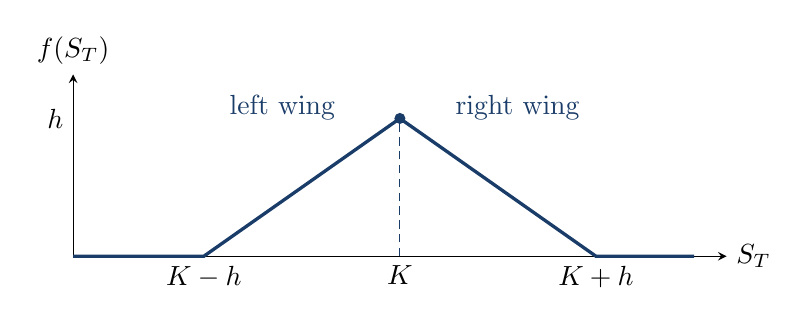
\begin{tikzpicture}[x=0.83cm,y=0.70cm,>=stealth]
  \draw[->] (0,0) -- (10,0) node[right] {$S_T$};
  \draw[->] (0,0) -- (0,3.3) node[above] {$f(S_T)$};
  \draw[CourseBlue,very thick] (0,0) -- (2,0) -- (5,2.5) -- (8,0) -- (9.5,0);
  \draw[CourseBlue,densely dashed] (5,0) -- (5,2.5);
  \node[below] at (2,0) {$K-h$};
  \node[below] at (5,0) {$K$};
  \node[below] at (8,0) {$K+h$};
  \node[left] at (0,2.5) {$h$};
  \node[above,CourseBlue] at (3.2,2.3) {left wing};
  \node[above,CourseBlue] at (6.8,2.3) {right wing};
  \fill[CourseBlue] (5,2.5) circle (2pt);
\end{tikzpicture}
\end{center}
\vspace{-0.4em}
\[
f(S_T)=(S_T-K+h)^+-2(S_T-K)^++(S_T-K-h)^+\geq0.
\]
\begin{marketbox}
The outer strikes form the wings; the payoff peaks at the middle strike.
Hence \(C_t(K-h)-2C_t(K)+C_t(K+h)\geq0\).
\end{marketbox}
\end{frame}

% ============================================================
\section{The Law of One Price}
% ============================================================

\begin{frame}{Identical payoffs must have identical prices}
Two self-financing strategies satisfy \(X_T=Y_T\) in every state.
\begin{pausebox}
If \(X_0\ne Y_0\), which strategy do you buy, and what are the cashflows?
\end{pausebox}
\pause
\begin{exampleblock}{Answer}
Buy the cheaper strategy and sell the more expensive one. Receive the price
gap today and owe \(X_T-Y_T=0\) at maturity. Therefore
\(\boxed{X_0=Y_0}\).
\end{exampleblock}
\end{frame}



\begin{frame}{Replication turns the law of one price into a pricing rule}
\begin{block}{Consequence for derivatives}
If a payoff \(H\) is replicated by a self-financing strategy with initial
cost \(X_0\), then no-arbitrage forces
\[
\boxed{V_0(H)=X_0.}
\]
\end{block}
\begin{exampleblock}{This is the bridge}
Everything we called ``martingale pricing'' in Lecture 7 is this statement,
combined with a convenient way of computing \(X_0\) as a conditional
expectation.
\end{exampleblock}
\end{frame}

\begin{frame}{Can you rebuild put--call parity from the law of one price alone?}
Compare a call plus \(K\) zero-coupon bonds with a put plus one share.
\begin{pausebox}
Compute both terminal payoffs. What must their current costs satisfy?
\end{pausebox}
\pause
\begin{exampleblock}{Answer}
\[
(S_T-K)^++K=(K-S_T)^++S_T=\max(S_T,K).
\]
The payoffs coincide, so \(\boxed{C_t+Ke^{-r(T-t)}=P_t+S_t}\).
\end{exampleblock}
\end{frame}



\begin{frame}{What does a call, a put, and two strikes always cost, together?}
For \(K_1<K_2\), buy \(C(K_1)\) and \(P(K_2)\), and sell \(C(K_2)\)
and \(P(K_1)\).
\begin{pausebox}
What is this box portfolio's payoff in each region of \(S_T\)?
\end{pausebox}
\pause
\begin{exampleblock}{Answer}
It pays \(K_2-K_1\) in every state, like a zero-coupon bond. Hence
\[
\boxed{C_t(K_1)-C_t(K_2)+P_t(K_2)-P_t(K_1)
=(K_2-K_1)e^{-r(T-t)}.}
\]
\end{exampleblock}
\end{frame}



% ============================================================
\section{Application: Pricing a Forward Contract}
% ============================================================

\begin{frame}{A forward payoff can be replicated with a bond and a share}
A forward pays \(S_T-K_t\). A zero-coupon bond costs \(P_t(T)\) and pays
\(1\) at \(T\). Assume no dividends.
\begin{pausebox}
Replicate the forward payoff. Which \(K_t\) makes its initial value zero?
\end{pausebox}
\pause
\begin{exampleblock}{Answer}
Buy one share and sell \(K_t\) bonds. Their cost is
\(S_t-K_tP_t(T)\), so
\[\boxed{K_t=\frac{S_t}{P_t(T)}.}\]
\end{exampleblock}
\end{frame}



\begin{frame}{What changes if the share pays a continuous dividend yield \(q\)?}
\begin{pausebox}
Reinvested dividends turn \(e^{-q(T-t)}\) shares today into one share at
\(T\). What is the zero-value forward delivery price?
\end{pausebox}
\pause
\begin{exampleblock}{Answer}
The prepaid share costs \(S_te^{-q(T-t)}\). Thus
\[
\boxed{F_{t,T}=\frac{S_te^{-q(T-t)}}{P_t(T)}};
\qquad
P_t(T)=e^{-r(T-t)}\ \Longrightarrow\
\boxed{F_{t,T}=S_te^{(r-q)(T-t)}}.
\]
\end{exampleblock}
\end{frame}



% ============================================================
\section{From No-Arbitrage to a Probability Measure}
% ============================================================

\begin{frame}{No-arbitrage has a probabilistic face}
\begin{block}{Informal principle}
A market is arbitrage-free precisely when there exists a probability measure
under which discounted traded asset prices are martingales. Such a measure
is called an equivalent martingale measure (EMM).
\end{block}
\begin{exampleblock}{Already familiar}
This is exactly the role \(\Q\) played in Black--Scholes: under \(\Q\),
\(D_tS_t\) is a martingale, and Girsanov is the tool that manufactures
\(\Q\) from \(\Pp\).
\end{exampleblock}
\end{frame}

\begin{frame}{Equivalence means \(\Q\) and \(\Pp\) agree on what is possible}
\[\Q\sim\Pp\quad\Longleftrightarrow\quad
  \Q\text{ and }\Pp\text{ have the same null events.}\]
\begin{pausebox}
Why must the martingale measure be equivalent to the historical measure?
\end{pausebox}
\pause
\begin{exampleblock}{Answer}
If \(\Pp(\omega)>0\) but \(\Q(\omega)=0\), \(\Q\) assigns zero value to a
payoff occurring only in that genuinely possible state. Equivalence prevents
pricing from ignoring such a risk.
\end{exampleblock}
\end{frame}



% ============================================================
\section{The First Fundamental Theorem of Asset Pricing}
% ============================================================

\begin{frame}{FTAP I: no-arbitrage and existence of an EMM are the same statement}
\begin{block}{First Fundamental Theorem, informal}
A financial market is arbitrage-free if and only if there exists an
equivalent martingale measure \(\Q\), under which every discounted traded
asset price is a \(\Q\)-(local) martingale.
\end{block}
\[
\boxed{
\text{no arbitrage}
\quad\Longleftrightarrow\quad
\text{an EMM exists}.}
\]
\end{frame}

\begin{frame}{One theorem, two languages}
\begin{center}
\begin{tabular}{p{0.42\textwidth}p{0.42\textwidth}}
\toprule
Economic statement & Probabilistic statement\\
\midrule
No free lunch from trading & An equivalent martingale measure exists\\
Prices are internally consistent & Discounted traded gains have no drift
under \(\Q\)\\
\bottomrule
\end{tabular}
\end{center}
\begin{exampleblock}{Why it matters}
The theorem lets us \emph{replace} a hard combinatorial search for arbitrage
strategies with an algebraic search for a consistent set of probabilities.
\end{exampleblock}
\end{frame}

\begin{frame}{Is this one-period market arbitrage-free?}
A stock has \(S_0=100\), factors \(u=1.2\), \(d=0.8\), and the bond has
gross return \(R=1.1\).
\begin{pausebox}
Find the up probability \(p\) that makes the discounted stock a
\(\Q\)-martingale. Is it a valid probability?
\end{pausebox}
\pause
\begin{exampleblock}{Answer}
\[
pu+(1-p)d=R
\quad\Longrightarrow\quad
\boxed{p=\frac{R-d}{u-d}=0.75\in(0,1).}
\]
An equivalent martingale measure exists. In general this requires
\(d<R<u\).
\end{exampleblock}
\end{frame}



\begin{frame}{What if the risk-free rate is too good, \(R=1.25>u\)?}
Keep \(S_0=100\), \(u=1.2\), and \(d=0.8\), but set \(R=1.25\).
\begin{pausebox}
Since no \(p\in(0,1)\) makes the discounted stock a martingale,
construct a zero-cost trade that profits in both states.
\end{pausebox}
\pause
\begin{exampleblock}{Answer}
Short one share for \(100\) and invest the proceeds in the bond.
At \(T\), receive \(125\), buy back the share, and keep
\[\boxed{125-S_T\in\{5,45\}>0.}\]
\end{exampleblock}
\end{frame}



\begin{frame}{A state price buys one dollar in one state}
The state claim \(e_k(\omega_j)=\1_{\{j=k\}}\) pays \(1\) only if
\(\omega_k\) occurs. Its positive state price \(\psi_k\) is today's cost
assigned to that payoff.
\[
\boxed{V_0(H)=\sum_{k=1}^K\psi_k H(\omega_k)}
\qquad\text{for every traded or attainable payoff }H.
\]
If a bond pays \(1\) at \(T\) and costs \(B_0=1/R\), then
\[
\sum_k\psi_k=B_0,\qquad q_k=R\psi_k>0,\qquad
\sum_k q_k=1.
\]
Thus \(V_0(H)=R^{-1}\E^\Q[H]\), where \(\Q(\omega_k)=q_k\).
\begin{block}{When a state claim is not traded}
The \(\psi_k\) are consistent shadow prices; they need not be unique in an
incomplete market.
\end{block}
\end{frame}

\begin{frame}{A bond and stock determine two state prices}
The bond pays \(1\) in each state and costs \(B_0=1/1.1\); the stock costs
\(100\) and pays \(120\) (up) or \(90\) (down).
\[
\psi_1+\psi_2=\frac1{1.1},
\qquad
120\psi_1+90\psi_2=100
\quad\Longrightarrow\quad
\boxed{\psi_1\approx0.6061,\ \ \psi_2\approx0.3030.}
\]
Both are positive. Multiplying by the bond return gives the risk-neutral
probabilities:
\[
q_{\mathrm{up}}=1.1\psi_1=\tfrac23,
\qquad q_{\mathrm{down}}=1.1\psi_2=\tfrac13.
\]
\begin{block}{Reading}
Each state price is a discounted risk-neutral probability:
\(\psi_k=B_0q_k\).
\end{block}
\end{frame}

\begin{frame}{Can a quoted stock price be inconsistent with the bond and the payoffs?}
A bond paying \(1\) costs \(B_0=1/1.1\). A stock quoted at \(115\) pays
\(120\) or \(90\) at maturity.
\begin{pausebox}
Solve for the two state prices. If one is negative, exhibit the trade.
\end{pausebox}
\pause
\begin{exampleblock}{Answer}
\(\psi_1+\psi_2=1/1.1\), \(120\psi_1+90\psi_2=115\) give
\(\psi_1\approx1.106\), \(\psi_2\approx-0.197\).
Short the stock for \(115\), buy \(120\) bonds for \(120/1.1\), and keep the
initial surplus. At \(T\), \(120-S_T\geq0\).
\end{exampleblock}
\end{frame}



% ============================================================
\section{The Second Fundamental Theorem of Asset Pricing}
% ============================================================

\begin{frame}{FTAP II: completeness and uniqueness of the EMM are the same statement}
\begin{block}{Second Fundamental Theorem, informal}
In an arbitrage-free market, the market is complete (every claim is
replicable) if and only if the equivalent martingale measure is unique.
\end{block}
\[
\boxed{
\text{market complete}
\quad\Longleftrightarrow\quad
\text{EMM unique}.}
\]
\begin{itemize}
  \item Unique EMM \(\Longrightarrow\) every replicable claim has one
        unambiguous price.
  \item Several EMMs \(\Longrightarrow\) no-arbitrage alone leaves a range of
        admissible prices for unreplicable claims.
\end{itemize}
\end{frame}

\begin{frame}{Does one bond and one stock pin down a three-state model?}
Let \(R=1.1\), \(S_0=100\), and \(S_T\in\{130,100,70\}\) in states
\((u,m,d)\).
\begin{pausebox}
Write the risk-neutral equations. Are the three probabilities unique?
\end{pausebox}
\pause
\begin{exampleblock}{Answer}
\[
p_u+p_m+p_d=1,
\qquad 1.3p_u+p_m+0.7p_d=1.1.
\]
With \(p_m=t\), the solutions are
\(\boxed{p_u=\tfrac23-\tfrac12t,\quad p_d=\tfrac13-\tfrac12t}\)
for \(0<t<2/3\): the EMM is not unique.
\end{exampleblock}
\end{frame}



\begin{frame}{Different EMMs price an unreplicable claim differently}
Take \(t=0.2\) and \(t=0.4\), both valid:
\[
t=0.2:\ (p_u,p_m,p_d)=(0.5667,\,0.2,\,0.2333),
\qquad
t=0.4:\ (0.4667,\,0.4,\,0.1333).
\]
\begin{pausebox}
Consider a claim paying \(1\) only in the middle state \(m\). Compute its
price under each measure. Do they agree?
\end{pausebox}
\pause
\[
\text{price}=\frac{p_m}{R}:
\qquad
\frac{0.2}{1.1}\approx0.182,
\qquad
\frac{0.4}{1.1}\approx0.364.
\]
Two legitimate EMMs, two different prices: no-arbitrage alone cannot select
one.
\end{frame}

\begin{frame}{Can a third traded asset restore completeness?}
In the three-state market, add a call paying \((30,0,0)\), quoted at
\(C_0\approx13.64\).
\begin{pausebox}
Use its pricing equation to find \(p_u\); then find \(p_m,p_d\).
\end{pausebox}
\pause
\begin{exampleblock}{Answer}
\[
\frac{30p_u}{1.1}=13.64
\quad\Longrightarrow\quad p_u\approx\tfrac12.
\]
The earlier two equations give
\(\boxed{(p_u,p_m,p_d)\approx(\tfrac12,\tfrac13,\tfrac16)}\).
The independent call payoff makes the EMM unique.
\end{exampleblock}
\end{frame}



\begin{frame}{Completeness is about spanning, not about counting assets}
\begin{block}{Why it worked}
The payoff vectors of the bond \((1,1,1)\), the stock \((1.3,1.0,0.7)\), and
the call \((30,0,0)\) are linearly independent: three genuinely different
exposures for three states.
\end{block}
\begin{marketbox}
This is literally why traders add options to a hedging book: a derivative
with a payoff the existing assets cannot replicate expands the span of
attainable claims, exactly as FTAP II predicts.
\end{marketbox}
\end{frame}

% ============================================================
\section{Superhedging and Price Bounds}
% ============================================================

\begin{frame}{When exact replication fails, dominance still gives bounds}
A self-financing strategy with wealth \(X\) \emph{superhedges} \(H\) if
\(X_T\geq H\) a.s.
\[
\boxed{V_0(H)\leq X_0.}
\]
A subhedging strategy \(Y_T\leq H\) gives a lower bound:
\[
\boxed{Y_0\leq V_0(H).}
\]
\begin{block}{Exact replication is the special case}
When \(X_T=H\) exactly, the upper and lower bounds coincide and
\(V_0(H)=X_0\).
\end{block}
\end{frame}

\begin{frame}{Parity plus positivity gives the call its lower bound for free}
We already derived \(C_t-P_t=S_t-Ke^{-r(T-t)}\) from the law of one price.
\begin{pausebox}
Combine this identity with \(P_t\geq0\) and \((S_T-K)^+\leq S_T\) to bound
\(C_t\) above and below, with no distributional assumption at all.
\end{pausebox}
\pause
\[
\boxed{
\bigl(S_t-Ke^{-r(T-t)}\bigr)^+\leq C_t\leq S_t.}
\]
\end{frame}

\begin{frame}{Can you bound a best-of-two-stocks claim without a model?}
Let \(H=\max(S_T^1,S_T^2)\), with nonnegative stock prices.
\begin{pausebox}
Which stock portfolio lies below \(H\), and which lies above it?
\end{pausebox}
\pause
\begin{exampleblock}{Answer}
Either single stock pays at most \(H\); holding both pays at least \(H\).
Dominance gives
\[
\boxed{\max(S_t^1,S_t^2)\leq V_t(H)\leq S_t^1+S_t^2.}
\]
\end{exampleblock}
\end{frame}



\begin{frame}{Can a digital option be bounded using only call prices?}
A digital pays \(D=\1_{\{S_T>K\}}\). For \(h>0\), compare it with the
bull spread at \(K,K+h\).
\begin{pausebox}
Does \(\bigl[(S_T-K)^+-(S_T-K-h)^+\bigr]/h\) lie above or below \(D\)?
\end{pausebox}
\pause
\begin{exampleblock}{Answer}
The spread pays \(0\), then \((S_T-K)/h\), then \(1\); it never exceeds
\(D\). Therefore
\[
\boxed{\frac{C_t(K)-C_t(K+h)}{h}\leq V_t(D).}
\]
\end{exampleblock}
\end{frame}



\begin{frame}{Can you build the matching superhedge?}
\begin{pausebox}
Compare the digital \(D=\1_{\{S_T>K\}}\) with the bull spread at
\(K-h,K\), scaled by \(1/h\). Which bound follows?
\end{pausebox}
\pause
\begin{exampleblock}{Answer}
This spread dominates \(D\), so its price is an upper bound. Together with
the previous slide,
\[
\boxed{\frac{C_t(K)-C_t(K+h)}{h}
\leq V_t(D)\leq
\frac{C_t(K-h)-C_t(K)}{h}.}
\]
\end{exampleblock}
\end{frame}



% ============================================================
\section{Synthesis}
% ============================================================

\begin{frame}{Four ideas, stacked in order}
\begin{enumerate}
  \item \textbf{No-arbitrage principles} (dominance, law of one price) rule
        out inconsistent prices, with no model.
  \item \textbf{Replication} gives an exact price whenever a payoff can be
        synthesized from traded assets.
  \item \textbf{Equivalent martingale measures} translate no-arbitrage into a
        probabilistic statement amenable to computation.
  \item \textbf{Completeness} determines whether that computation returns one
        price or only a range.
\end{enumerate}
\end{frame}

\begin{frame}{The big picture in one line}
\[
\boxed{
\text{no-arbitrage}
\quad\Longleftrightarrow\quad
\text{martingale pricing under a suitable measure.}}
\]
\begin{block}{This lecture versus Lecture 7}
Lecture 7 \emph{used} an EMM to price and hedge. Today explains its existence
(FTAP I), its uniqueness (FTAP II), and the bounds that remain when
replication is unavailable.
\end{block}
\end{frame}

\begin{frame}{Can you diagnose an arbitrage from raw quotes?}
For one maturity, suppose \(C_t(90)=14\), \(C_t(100)=12\), and
\(C_t(110)=7\).
\begin{pausebox}
Check strike monotonicity and convexity. Construct the trade if a quote
violates either condition.
\end{pausebox}
\pause
\begin{exampleblock}{Answer}
Monotonicity holds, but convexity requires
\(C_t(100)\leq(14+7)/2=10.5<12\).
Buy the wings and sell two middle calls: cost \(14+7-2(12)=-3\), while the
butterfly payoff is nonnegative in every state.
\end{exampleblock}
\end{frame}





\begin{frame}{Five checks before trusting a claimed no-arbitrage price}
\begin{enumerate}
  \item Is the comparison payoff actually dominating, in \emph{every} state?
  \item Is the replicating strategy genuinely self-financing?
  \item Is the candidate pricing measure equivalent to \(\Pp\), not merely a
        probability measure?
  \item Is the EMM unique for this market, or only for the traded assets?
  \item If replication fails, have you produced \emph{both} a superhedge and
        a subhedge, not just one?
\end{enumerate}
\begin{marketbox}
Dominance, the law of one price, and the two Fundamental Theorems are the
same idea seen at four levels of abstraction.
\end{marketbox}
\end{frame}

\end{document}
